\documentclass[11pt,a4paper]{report}

\usepackage{fullpage}
\usepackage{fancyhdr}
\usepackage{lastpage}
\usepackage{mathtools}
\usepackage{gensymb}
\usepackage{fontspec}
\usepackage{color}
\usepackage{graphicx}
\usepackage{wrapfig}
\usepackage{tabularx}
\usepackage{hyperref}
\usepackage[french]{babel}
\usepackage{indentfirst}
\usepackage{multicol}
%\usepackage{float}
\usepackage{mdwlist}
%\usepackage{bnf}
\usepackage{listliketab}
\usepackage[export]{adjustbox}
\usepackage{subfigure}


% for languages codes
\usepackage{xcolor}
\usepackage{listings}
\renewcommand{\lstlistingname}{Extrait de code}
\lstset{basicstyle=\ttfamily,
  showstringspaces=false,
  commentstyle=\color{gray},
  keywordstyle=\color{blue}
}
% https://tex.stackexchange.com/questions/89574/language-option-supported-in-listings
\lstdefinelanguage{javascript}{
  keywords={typeof, new, true, false, catch, function, return, null, catch, switch, var, if, in, while, do, else, case, break},
  keywordstyle=\color{blue}\bfseries,
  ndkeywords={class, export, boolean, throw, implements, import, this},
  ndkeywordstyle=\color{darkgray}\bfseries,
  identifierstyle=\color{black},
  sensitive=false,
  comment=[l]{//},
  morecomment=[s]{/*}{*/},
  commentstyle=\color{gray}\ttfamily,
  stringstyle=\color{green}\ttfamily,
  morestring=[b]',
  morestring=[b]"
}


\newcommand\vartitle{Étude sur l'apprentissage par renforcement dans les jeux \\Projet de Bachelor - hepia}
\newcommand\varauthor{Federico Pfeiffer}
\newcommand\vardate{\today}

\title{\vartitle}
\author{\varauthor}
\date{\vardate}

% page layout
\pagestyle{fancyplain}
\lhead[\vartitle]{\vartitle}
\chead[]{}
\rhead[\varauthor]{\varauthor}
\lfoot[]{}
\cfoot[\thepage\ of \pageref{LastPage}]{\thepage\ of \pageref{LastPage}}
\rfoot[]{}

\renewcommand{\headrulewidth}{0.2mm}
\renewcommand{\footrulewidth}{0mm}

\setlength{\headsep}{40pt}
\setlength{\voffset}{0cm}
\setlength{\topmargin}{-1.7cm}
\setlength{\textheight}{730pt}

\setlength{\columnsep}{30pt}

\setlength{\parindent}{0mm}
\setlength{\parskip}{2mm}

% only chapters / sections / subsections are numbered 
\setcounter{secnumdepth}{2}

% only chapters / sections are in table of contents
\setcounter{tocdepth}{1}



\hypersetup{
  hidelinks,
  pdfstartview={FitV},
  pdftitle={\vartitle},
  pdfauthor={\varauthor}
}

\begin{document}

  \begin{titlepage}
    \maketitle

    \thispagestyle{empty}

    \begin{abstract}
    // TODO
    \end{abstract}

%    \vspace{1cm}

  \end{titlepage}
  
  \newpage
  
  \tableofcontents
  
  \newpage

  \chapter{Introduction}
  
  \chapter{Théorie}
  
  \section{Notions de base}
  
  \subsection{Fonctionnement général de l'apprentissage par renforcement}
  
    \par L'apprentissage par renforcement consiste à donner une récompense à un agent lorsque ce dernier parvient à effectuer une tâche demandée, ou lorsqu'il s'en approche. De la même manière, l'agent reçoit un malus lorsque ce dernier s'éloigne de la tâche demandée. Le but de l'agent est d'obtenir un maximum de récompense. De cette manière, le comportement de l'agent est influencé par les récompenses et malus qu'il reçoit. Au fur et à mesure que l'agent effectue des actions et reçoit des récompenses/malus, ce dernier tend à renforcer un comportement menant à un maximum de récompenses, et éviter les actions menant à des malus. À noter qu'à partir de maintenant nous ne parlerons que de récompenses: un malus sera simplement traduit par une récompense négative. 
  
    \par Plus concrètement, l'agent commence par effectuer des actions aléatoires et reçoit une récompense / malus pour chaque action effectuée. Pour chaque action commise, l'agent enregistre l'état $S$ dans lequel il se trouvait, l'action effectuée, la récompense/malus reçue  et l'état $S'$ dans lequel il se retrouve suite à l'action. Si l'agent se retrouve dans un état terminal, l'environnement est réinitialisé mais l'agent garde en mémoire les actions / états / récompenses vécus. À une fréquence définie par le développeur, l'agent passe par une phase d'ajustement \textit{(training)} où il parcourt tous les actions / états / récompenses vécus de sorte à ajuster son comportement (actions choisies) lors des états futurs qu'il rencontrera, dans le but de maximiser les récompenses. 

  \subsection{Valeur d'un état}
  
    \par Jusqu'à la fin du chapitre, nous définirons le score d'un épisode par la somme des récompenses obtenues au cours des actions effectuées. Le but de l'agent est d'obtenir le meilleur score possible, et de retenir les états par lesquels il est passé afin d'obtenir ce meilleur score. (Et également de retenir les états par lesquels il est passé qu'il l'ont mené à un mauvais score). 
    
    \par Afin d'apprendre à choisir les bonnes actions à effectuer en fonction de l'état où l'agent se trouve, ce dernier a pour but d'apprendre la valeur de chaque état qu'il rencontre: un état qui le rapproche d'un meilleur score a une meilleure valeur qu'un état qui l'éloigne d'un meilleur score. 
    
    \par L'enjeu est donc de trouver une manière d'attribuer une valeur à chaque état en fonction des états qui vont suivre, afin de choisir l'action appropriée menant à un meilleur état. Prenons l'exemple (arbitraire) comprenant 2 épisodes, avec un état initial s0 \textit{(s pour state)}: 
    
    \begin{figure}[!h]
    \center
    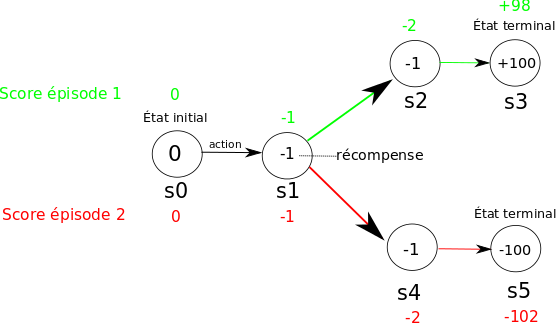
\includegraphics[scale=0.60]{ressources/introduction_function_value.png}
    \caption{Valeur d'un état: introduction 1}
    \end{figure} 
    
    \par Dans le premier épisode, l'agent commence à l'état s0 (état initial), puis choisit les actions passant par s1, s2 et s3. s3 étant un état terminal, l'épisode 1 s'arrête et l'agent obtient comme score +98 (qui est la somme des récompenses obtenues pendant son épisode). Dans le deuxième épisode, l'agent commence à l'état s0 (état initial), puis choisit les actions passant par s1, s4 et s5. s5 étant un état terminal, l'épisode 2 s'arrête et l'agent obtient un score de -102 pour le deuxième épisode. 
    
    \par Comment pourrions-nous donc attribuer une valeur à chaque état? Intuitivement, nous concluons qu'il est nécessaire d'attribuer une valeur à chaque état une fois qu'un épisode est terminé. En effet, une fois l'épisode terminé, nous pouvons évaluer chacune des actions prises par l'agent, étant donné que nous savons si les actions effectuées ont mené à l'état terminal voulu. Une première idée serait donc d'attribuer à chaque état la récompense finale auquel l'état peut mener. Si un état mène à deux récompenses différentes, nous pouvons par exemple attribuer la valeur de l'état en faisant la somme des deux récompenses auxquels l'état peut mener. 
    
    \begin{figure}[!h]
    \center
    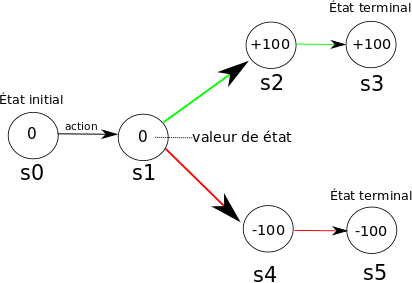
\includegraphics[scale=0.60]{ressources/introduction_function_value_2.png}
    \caption{Valeur d'un état: introduction 2}
    \end{figure}
    
    \par Après avoir effectué sa phase d'ajustement \textit{(training)} dans le but de connaître la valeur de chaque état (phase d'apprentissage), l'agent peut ensuite savoir que depuis l'état s1, il est préférable de choisir l'action menant à l'état s2, étant donné qu'un meilleur score l'attend.
    
\subsubsection{Discount factor ($\gamma$)}
  
    \par Le problème de la méthode précédente pour attribuer une valeur à un état est qu'on ne tient pas compte de la distance à laquelle se trouve la récompense finale.\\
    En prenant l'exemple suivant, il serait préférable pour l'agent de passer directement à s3 depuis s1. (L'agent a meilleur temps d'effectuer l'action qui le mène le plus rapidement à l'état menant à une forte récompense). Or, l'agent n'a pas de moyen de savoir qu'il a meilleur temps de passer directement par s3:
    
    \begin{figure}[!h]
    \center
    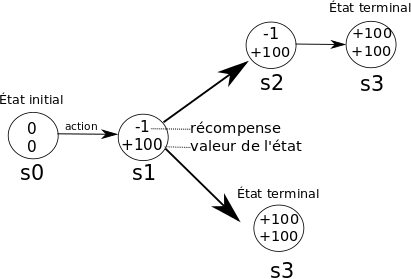
\includegraphics[scale=0.60]{ressources/introduction_function_value_3.png}
    \caption{Valeur d'un état: introduction sans discount factor}
    \end{figure}
    
    \par Une solution pour palier à ce problème est de calculer la valeur d'un état en ajoutant un coefficient nommé \textit{discount factor} $\gamma$ de cette manière: $V(s_t) = \gamma V(s_{t+1})$ avec $\gamma \in [0,1]$. En prenant $\gamma = 0.9$, on parvient à attribuer une valeur à chaque état qui inclut cette notion de distance envers la récompense la plus forte. Depuis s1, l'agent va donc tendre vers s3 directement car la valeur de s3 est plus grande que s2.
    
    \begin{figure}[!h]
    \center
    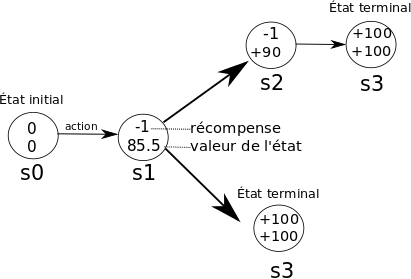
\includegraphics[scale=0.60]{ressources/introduction_function_value_4.png}
    \caption{Valeur d'un état: introduction avec discount factor}
    \end{figure} 
    
  \subsection{V(s): Équation de Bellman}
  
    \par La fonction $V(s) = \gamma V(s_{t+1})$ est incomplète. La version formelle vient de l'équation de Bellman. Elle prends en compte plusieurs notions  supplémentaires: 
    
    \par Elle prends en compte la récompense reçue à chaque état, ce qui donne \\ $V(s_t) = r + \gamma V(S_{t+1})$
    
    \par Aussi, il est possible qu'un environnement soit fait de telle sorte qu'une transition d'un état à un autre ne soit pas déterministe. Par exemple, si un agent choisit une action menant à un état $S'$, on peut imaginer que l'environnement aie un comportement aléatoire menant l'agent à un état qui n'était pas prévu par l'agent. (dans l'exemple d'une voiture autonome, le fait de voir un enfant jouer sur un trottoir n'implique pas forcément que celui-ci reste sur le trottoir). Pour un état $s_t$, il faudrait pouvoir multiplier la probabilité de se retrouver dans un état $s_{t+1}$, et recevoir une récompense $r$ après avoir fait une action $a$. En d'autres termes, pour un état $s_t$, il faut évaluer tous les états $s_{t+1}$ et toutes les récompenses $r$, et en calculer la probabilité. \\
    La fonction V(s) devient $$\sum_{s_{t+1}}\sum_rp(s_{t+1},r\ |s_t,a)\left\{r+\gamma V(s_{t+1})\right\}$$
    
    \par Enfin, il se peut pour un certain état, l'agent aie une certaine probabilité de choisir une certaine action. (Il peut par exemple connaître la meilleur action à entreprendre, mais il a une politique d'avoir 10\% de probabilité de faire une action aléatoire dans le but d'explorer certaines actions). La fonction est alors agrémentée du terme suivant: $\sum_a\pi(a|s)$. Le $\pi$ représente la politique de l'agent.
    
    \par Ainsi, l'équation de Bellman indique que la valeur d'un état peut se calculer de la manière suivante: 
    
    $$V_\pi(s) = \sum_a\pi(a|s)\sum_{s'}\sum_rp(s',r\ |s,a)\left\{r+\gamma V_\pi(s')\right\}$$
    
    \par Le terme $\pi(a|s)$ représente la probabilité de choisir une action $a$ étant donné l'état $s$, suivant une politique $\pi$. (Dans le cas où la politique de l'agent est de choisir une action aléatoire tous les 10\% par exemple). Si l'agent a une politique visant à ne choisir que la meilleure action et que le choix de cette action n'est pas probabiliste, ce terme vaut simplement 1. De même, si l'agent n'a qu'une action possible pour un certain état $s$, le terme $\sum_a\pi(a|s)$ équivaut à $\pi(a|s)$
    
    \par Le terme $p(s',r\ |s,a)$ représente, depuis un état $s$, la probabilité de se retrouver dans l'état suivant $s'$ et de gagner la récompense $r$, ayant choisi l'action $a$. Pour connaître la valeur de l'état $s$, il faut donc pouvoir envisager tous les états $s'$ possibles, et toutes les récompenses $r$ en choisissant une action $a$. C'est pour cela que l'on "itère" en faisant la somme de tous les $p(s',r\ |s,a)$ en parcourant tous les états $s'$ possibles et toutes les récompenses $r$ possibles depuis un état $s$. D'où les deux sommes $\sum_{s'}\sum_r$ devant $p(s',r\ |s,a)$:  $\sum_{s'}\sum_rp(s',r\ |s,a)$
    
    \par L'équation de Bellman peut être lue de la manière suivante: depuis un état $s$, on itère toutes les actions possibles depuis cet état. Dans cette itération, on itère toutes les récompenses possibles et tous les états $s'$ qui découlent en choisissant l'action $a$. A chaque itération, on multiplie la probabilité $\pi(a|s)$ à la probabilité $p(s',r\ |s,a)$ et multiplie à la $\left\{r+\gamma V_\pi(s')\right\}$
    
    $$V_\pi(s) = \sum_a\pi(a|s)\sum_{s'}\sum_rp(s',r\ |s,a)\left\{r+\gamma V_\pi(s')\right\}$$
    
    \par Dans ce projet de bachelor, nous considérerons l'environnement déterministe, ce qui réduit l'équation de Bellman à ceci: 
    
    $$V_\pi(s) = \sum_a\pi(a|s)\left\{r+\gamma V_\pi(s')\right\}$$
    
    \par De même, nous considérerons que lorsque un agent choisit d'effectuer une action, celle-ci sera réalisée, réduisant l'équation de Bellman à ceci: 
    
    $$V_\pi(s) = r+\gamma V_\pi(s')$$
    
  \subsection{Apprentissage par renforcement: pseudo code}
  
  \par Maintenant que nous connaissons comment attribuer une valeur à chaque état, nous pouvons imaginer un premier pseudo-code permettant à un agent d'apprendre à évoluer dans un environnement. Le problème de cette équation est qu'elle part du principe que nous connaissons tous les états et actions possibles. Il faut donc procéder de manière itérative jusqu'à ce que la valeur d'un état converge vers une valeur fixe. Nous nous arrêtons lorsque toutes les valeurs des états semblent avoir été calculées:  
  
   \begin{lstlisting}[language=python]
 
  # phase d'apprentissage
  world = new World()
  agent = new Agent()
  gamma = 0.9
  
  max_divergence = 0.1
  divergence = inf
  while divergence > max_divergence:
    for state in world.get_all_states():
      for action in world.get_possible_actions(state):
        reward, next_state = world.do_action(state, action)
        old_v = agent.V[state]
        agent.V[state] = reward + gamma * agent.V[next_state]
        divergence = max(divergence, abs(old_v-agent.V[state]))
        
  # phase une fois l'apprentissage effectué
  state = world.reset()
  while not world.is_in_terminal_state():
    action = agent.choose_action_to_best_state(state)
    state = world.do_action(action)
        
   \end{lstlisting}
  
  \par Enfin, l'équation de Bellman suppose donc que l'on connaisse tous les états possibles et toutes les actions possibles pour chaque état. Ceci pose évidemment problème dans le cas de l'apprentissage par renforcement, étant donné que l'agent doit apprendre en explorant lui-même à travers les actions qu'il entreprend. Pour des raisons de temps de calcul, nous ne souhaitons pas explorer toutes les actions possibles, mais souhaitons explorer que celles qui nous semblent nous mener à un meilleur comportement de l'agent. Heureusement, des algorithmes ont été mis en place afin de pouvoir estimer correctement la fonction de Bellman ($V(s)$) sans avoir à tout explorer, permettant ainsi à l'agent de pouvoir estimer raisonnablement la valeur de l'état dans lequel il se trouve, et choisir l'action adéquate pour maximiser son score. 
    
  \section{Algorithme Q-Learning}
  
  \subsection{Explore vs Exploit} 
  
    \par Dans la précédente section, nous avons vu un algorithme permettant d'évaluer V(s) en supposant que l'on connaisse tous les états, actions et récompenses possibles suivant l'environnement donné. Dans la majorité des cas, il n'est évidemment pas possible de connaître toutes ces valeurs à l'avance. Il convient donc d'utiliser l'agent de sorte à ce qu'il explore de lui même toutes ces différentes valeurs dans le but d'estimer correctement la fonction V(s).     
    
    \par Au fur et à mesure que l'agent explore les actions, la fonction V(s) va petit à petit atteindre une estimation correcte, et l'agent va petit à petit connaître les meilleurs états à rencontrer, ou les meilleures actions à effectuer pour chaque état. 
    
    \par Comment savoir si l'agent dispose de connaissances suffisantes pour arrêter d'explorer/tester des actions? A quel moment l'agent doit-il utiliser la connaissance qu'il dispose de V(s)? Une solution est d'effectuer une action aléatoire avec une probabilité $\epsilon$. La valeur de $\epsilon$ peut varier en fonction du temps selon ce qu'a choisit le programmeur. 
  
  \subsection{Valeur d'un état avec Q(s,a)}
  
    \par Utiliser V(s) pour attribuer une valeur à chaque état peut s'avérer limitant: on n'enregistre finalement que la valeur d'un état en fonction de l'état en question. Au lieu d'attribuer une valeur à un état, nous pourrions attribuer une valeur à un couple état/action effectué. 
    
    \par La fonction attribuant une valeur à un couple état/action s'appelle la fonction Q value, ou Q(s,a), et peut être représentée de la sorte, ressemblant fortement à V(s): 
        
    \begin{eqnarray}
      V_\pi(s) &=& \sum_a\pi(a|s)\sum_{s'}\sum_rp(s',r\ |s,a)\left\{r+\gamma V_\pi(s')\right\} \\
      Q_\pi(s,a) &=& \sum_{s'}\sum_rp(s',r\ |s,a)\left\{r+\gamma Q_\pi(s',a')\right\}
    \end{eqnarray}
    
    \par Comme indiqué plus haut, l'environnement utilisé est déterministe, ce qui permet de réduire les équations à ceci: 
    
    \begin{eqnarray}
      V_\pi(s) &=& \sum_a\pi(a|s)\left\{r+\gamma V_\pi(s')\right\} \\
      Q_\pi(s,a) &=& \left\{r+\gamma Q_\pi(s',a')\right\}
    \end{eqnarray}
    
  \subsection{Algorithme Q-Learning}
  
   \par Si nous connaissions tous les états, actions et récompenses possibles, il serait possible de définir Q(s,a) dans un environnement déterministe, de la manière suivante: 
    $$Q(s,a) = r +  \gamma Q(s',a')$$
    Or, ne connaissant pas tous les états, actions et récompenses possibles, (et ne voulant pas tous les explorer), l'idée du Q-learning est d'ajuster petit à petit Q(s,a), par une fraction $\alpha$.  
    $$Q(s,a) = old\_Q(s,a) + \alpha(new\_Q(s,a) - old\_Q(s,a))$$
    Le terme $\alpha$ est appelé "learning\_rate" est choisi arbitrairement par le développeur et est compris entre $[0,1]$. Il correspond à l'$\alpha$ utilisé lors d'un "gradient descent". 
    
    \par La méthode Q-Learning met donc Q(s,a) à jour selon la formule suivante: 
    $$Q(s,a) = Q(s,a) + \alpha(\left\{  r + \gamma Q(s', a') \right\} - Q(s,a) )$$  
    
    \par Le pseudo-code de la méthode Q-learning peut être défini de la manière suivante: 
  
   \begin{lstlisting}[language=python]
 
  # phase d'apprentissage
  world = new World()
  agent = new Agent()
  max_episodes = 100000
  gamma = 0.9
  epsilon = 0.1
  alpha = 0.1
  
  for i in range(max_episodes):
    state = world.reset()
    while not world.game_over():
      action = agent.choose_action(state, epsilon)
      reward, next_state = world.do_action(state, action)
      a2 = agent.choose_action(next_state, epsilon)
      agent.Q[state][action] += alpha*(reward+gamma*agent.Q[next_state][a2])
      state = next_state
    
        
  # phase une fois l'apprentissage effectué
  state = world.reset()
  while not world.game_over():
    action = agent.choose_action(state, epsilon)
    state, _ = world.do_action(action)
        
   \end{lstlisting} 
    
  \subsection{Limitations de l'algorithme Q-Learning}
    
    \par L'inconvénient majeur de l'algorithme Q-Learning vient du fait qu'il faut pouvoir stocker la fonction Q(s,a) dans un tableau représentant chaque couple (état, action): si le fait de garder en mémoire V(s) utilise un tableau à 1 dimensions de taille équivalant à autant d'états possibles, la fonction Q(s,a) nécessite beaucoup plus de mémoire car elle doit enregistrer les valeurs dans un tableau à 2 dimensions, de taille $|S| * |A|$ cases. 
    
    \begin{figure}[!h]
    \center
    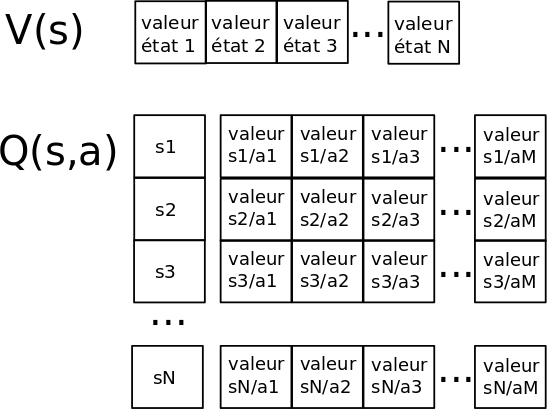
\includegraphics[scale=0.45]{ressources/v_s_vs_q_sa.png}
    \caption{Enregistrement V(s) et Q(s,a)}
    \end{figure} 
    
   \par Dans des environnements avec de nombreux (voir infinités) d'états et d'autant d'actions possibles, le stockage de la valeur de Q(s,a) devient très difficile vu la taille qu'elle représente. De plus, si l'environnement présente autant d'états et d'action possibles, l'agent va devoir effectuer beaucoup d'exploration afin d'évaluer la valeur de chaque couple (état, action), ce qui rendrait l'apprentissage extrêmement lent, voir impossible. Une solution pour palier à cet inconvénient est de remplacer le tableau Q[s][a] par un réseau neuronal. 
   
  \section{Réseaux neuronaux}
  
  \chapter{Conception}
  
  \chapter{Résultats}
  
  \chapter{Annexes}
       
\end{document}
